% !Mode:: "TeX:UTF-8"
%%% Local Variables:
%%% mode: latex
%%% TeX-master: t
%%% End:

\chapter{遥感影像识别分类基础方法介绍}
\label{cha:chap02}
%目标地物的识别分类一直是遥感影像解译中的重大任务。遥感影像分类任务依据是否使用地物类别先验知识分为监督分类和非监督分类。由于遥感影像多以非结构化、不精确的形式存在,缺乏完善的标记类别的规整数据。传统影像分割识别方法多以无监督的聚类分割辅以人工后处理的方法来完成遥感影像的解译工作。遥感影像数据固有的不确定性(“混合像元”、“同物异谱”和“同谱异物”等)使得模糊C-均值聚类方法成为遥感影像无监督聚类分割的优选方法,被广泛应用到遥感影像聚类分割识别任务中\cite{he2016remote}。另一方面,深度神经网络因其在特征提取方面效果显著,能够较好提取遥感影像复杂数据结构的隐含特征信息。并且,基于生成对抗网络模型的神经网络模型能够解决遥感影像分割中样本数不足的问题,因此具有重要的研究意义。

本课题主要从表征影像不确定性和小样本影像数据分类两个方面来研究遥感影像的分类识别方法。第~\ref{cha:chap03} 章研究内容是对当前的模糊聚类遥感影像无监督分割方法改进,能够更好地表达遥感影像“同物异谱”的不确定性;这部分工作基于遥感影像的模糊聚类分割基础知识;第~\ref{cha:chap04} 章则是结合深度神经网络相关方法,针对少标签样本的影像数据,提出基于生成对抗网络框架的遥感影像分割方法,该章节中的大量工作将基于深度学习中的卷积神经网络和图像语义分割相关的知识。所以本章将依次介绍遥感影像模糊聚类无监督分割方法,神经网络基础知识以及深度神经网络用于影像分割的网络设计方法和思想。

\section{遥感影像的模糊聚类分割基础}
\label{sec:chap02-1}
本课题中处理的遥感影像数据均为高分辨率遥感影像数据,文中主要研究面向对象的遥感影像模糊聚类方法。面向对象的模糊聚类方法主要包含影像分割,模糊聚类和后处理三个部分。

\subsection{影像分割方法}
\label{subsec:chap02-1-1}
面向对象的影像分割是指对遥感影像分割划分,将邻域内同质性的像元当作一个整体,形成的影像分割单元区域内部的颜色、灰度、纹理等特性相似性较大,区域间的颜色、灰度、纹理等特性相异性较大。常见的影像分割根据分割类型可以划分为:边缘检测分割方法、阈值分割方法和基于区域的分割方法。边缘检测分割方法是通过Sobel、Canny、LOG 等滤波算子提取影像边缘,再将边缘连接起来形成边界,一般适用于灰度影像的分割。阈值分割方法通过比较像素与设定阈值大小关系,划分影像的前景和背景,该方法简单但不适用于较复杂的影像。基于区域的分割方法包含生长法和区域分裂合并法,其原理依据是影像中距离近的像素点相似性大,距离远的相似性小。基于区域的分割方法应用广泛,且分割效果较好。文中详细介绍两种常见的分割方法:Watershed 分水岭算法\cite{vincent1991watersheds} 和SLIC 超像素分割算法\cite{achanta2012slic}。

\subsubsection{Watershed 分水岭算法}
\label{subsubsec:chap02-1-1-1}
Watershed 分水岭分割算法是一个非常经典的区域生长分割方法。算法的思想是把待分割图像想象成一个地理上的地形图,图像灰度值大小可看作地形高程值,图像每个局部极小值及其影响区域对应地形上的低洼处,即集水盆。两个集水盆汇合边界则为分水岭。分水岭算法如图~\ref{fig:watershed} 所示。

\begin{figure}[htb]
  \centering
  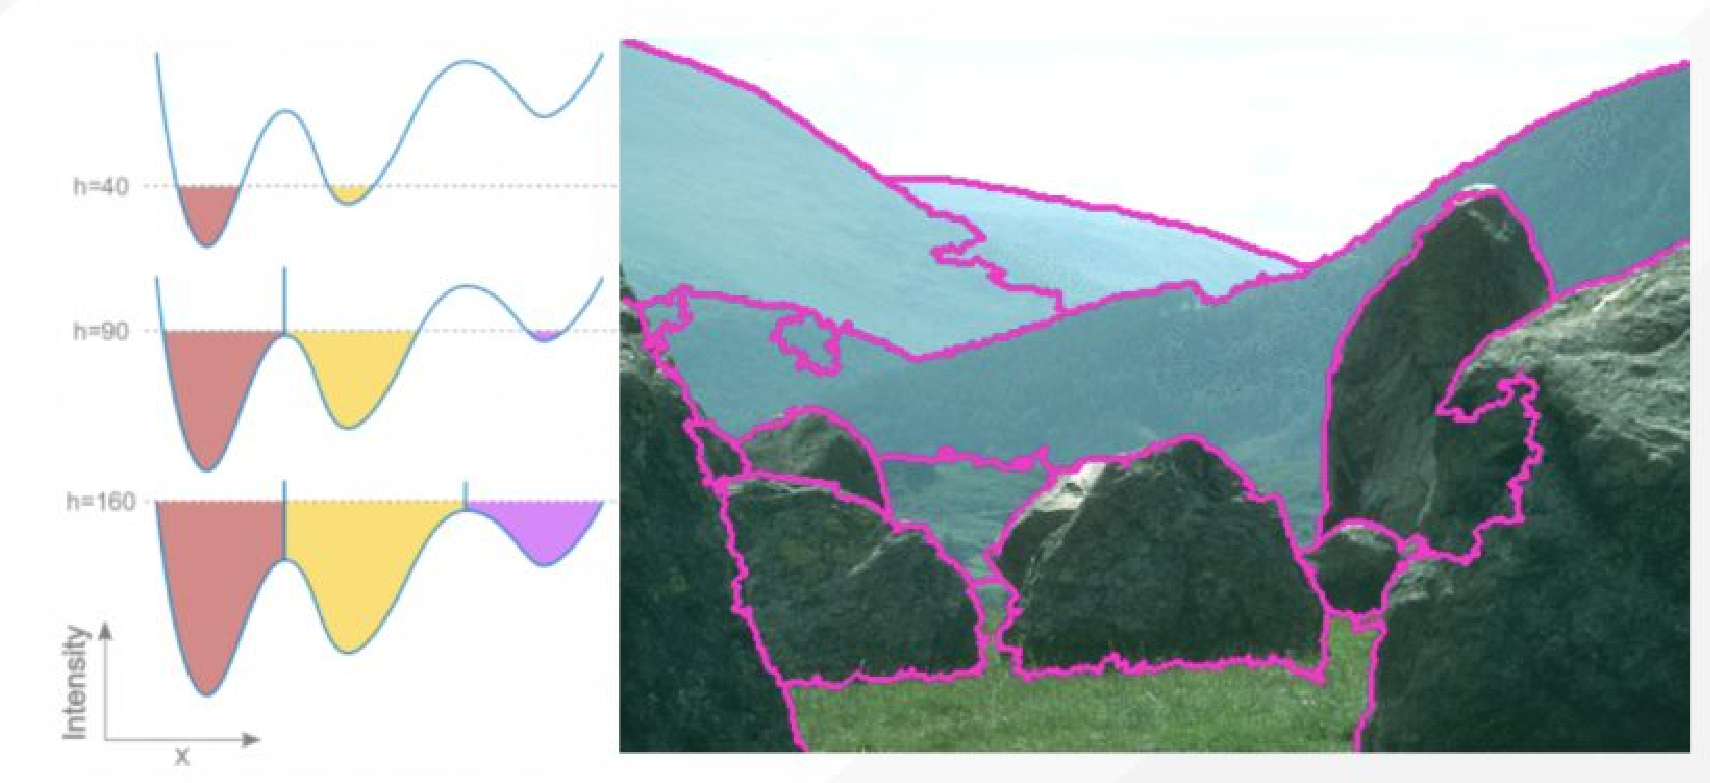
\includegraphics[width=0.7\textwidth]{figures/watershed}
  \caption{Watershed 分水岭算法示意图 }\label{fig:watershed}
\end{figure}

根据Watershed 分水岭算法原理,为得到图像的边缘信息,通常把梯度图像作为输入图像,即
\begin{equation}
  \label{eq:2-1}
  g(x,y) = \nabla f = \left[
    \begin{matrix}
      G_x \\
      G_y
    \end{matrix}
    \right] =
  \left[
    \begin{matrix}
      \frac{\partial f}{\partial x} \\
      \frac{\partial f}{\partial y}
    \end{matrix}
    \right]
\end{equation}
其中,$f(x,y)$表示原始图像,$g(x,y)$ 表示原始图像的梯度运算。假设$R_1,R_2,R_3,\cdots,R_m$ 表示待分割图像的极小区域的集合,$C(R_i)$ 表示为与极小区域$R_i$ 相关的流域,$n$ 表示溢流的增加数值(即在第$n$ 步时溢流的深度),$T[n]$ 表示满足梯度$g(x,y)<n$ 的所有像素点$(x,y)$ 的集合。对于一个给定流域,假设在第$n$ 步时极小区域$R_i$ 发生溢流,令$C_n(R_i)$ 为与极小区域$R_i$ 相关流域的一部分,即在溢流深度$n$ 时,在流域$C(R_i)$ 中形成的水平面构成的区域,$C_n(R_i)$ 为二值图像,可表示为:
\begin{equation}
  \label{eq:2-2}
  C_n(R_i) = C(R_i)\cup T[n]
\end{equation}
为防止分水岭算法产生的过度分割,通常设置阈值对梯度函数进行修改,以消除灰度的微小变化产生的过度分割。即
\begin{equation}
  \label{eq:2-3}
  g(x,y) = \max ( \nabla f(x,y),g_{\theta})
\end{equation}
式中,$g_{\theta}$ 表示阈值。

\subsubsection{SLIC 超像素分割算法}
\label{subsubsec:chap02-1-1-1}
SLIC(Simple linear iterativeclustering),即简单的线性迭代聚类超像素分割方法。它采用$K$ 均值聚类方法高效地生成超像素,较以前的算法可以更好地获取分割边界,且有着更快的运行速度。

\begin{figure}[htb]
  \centering
  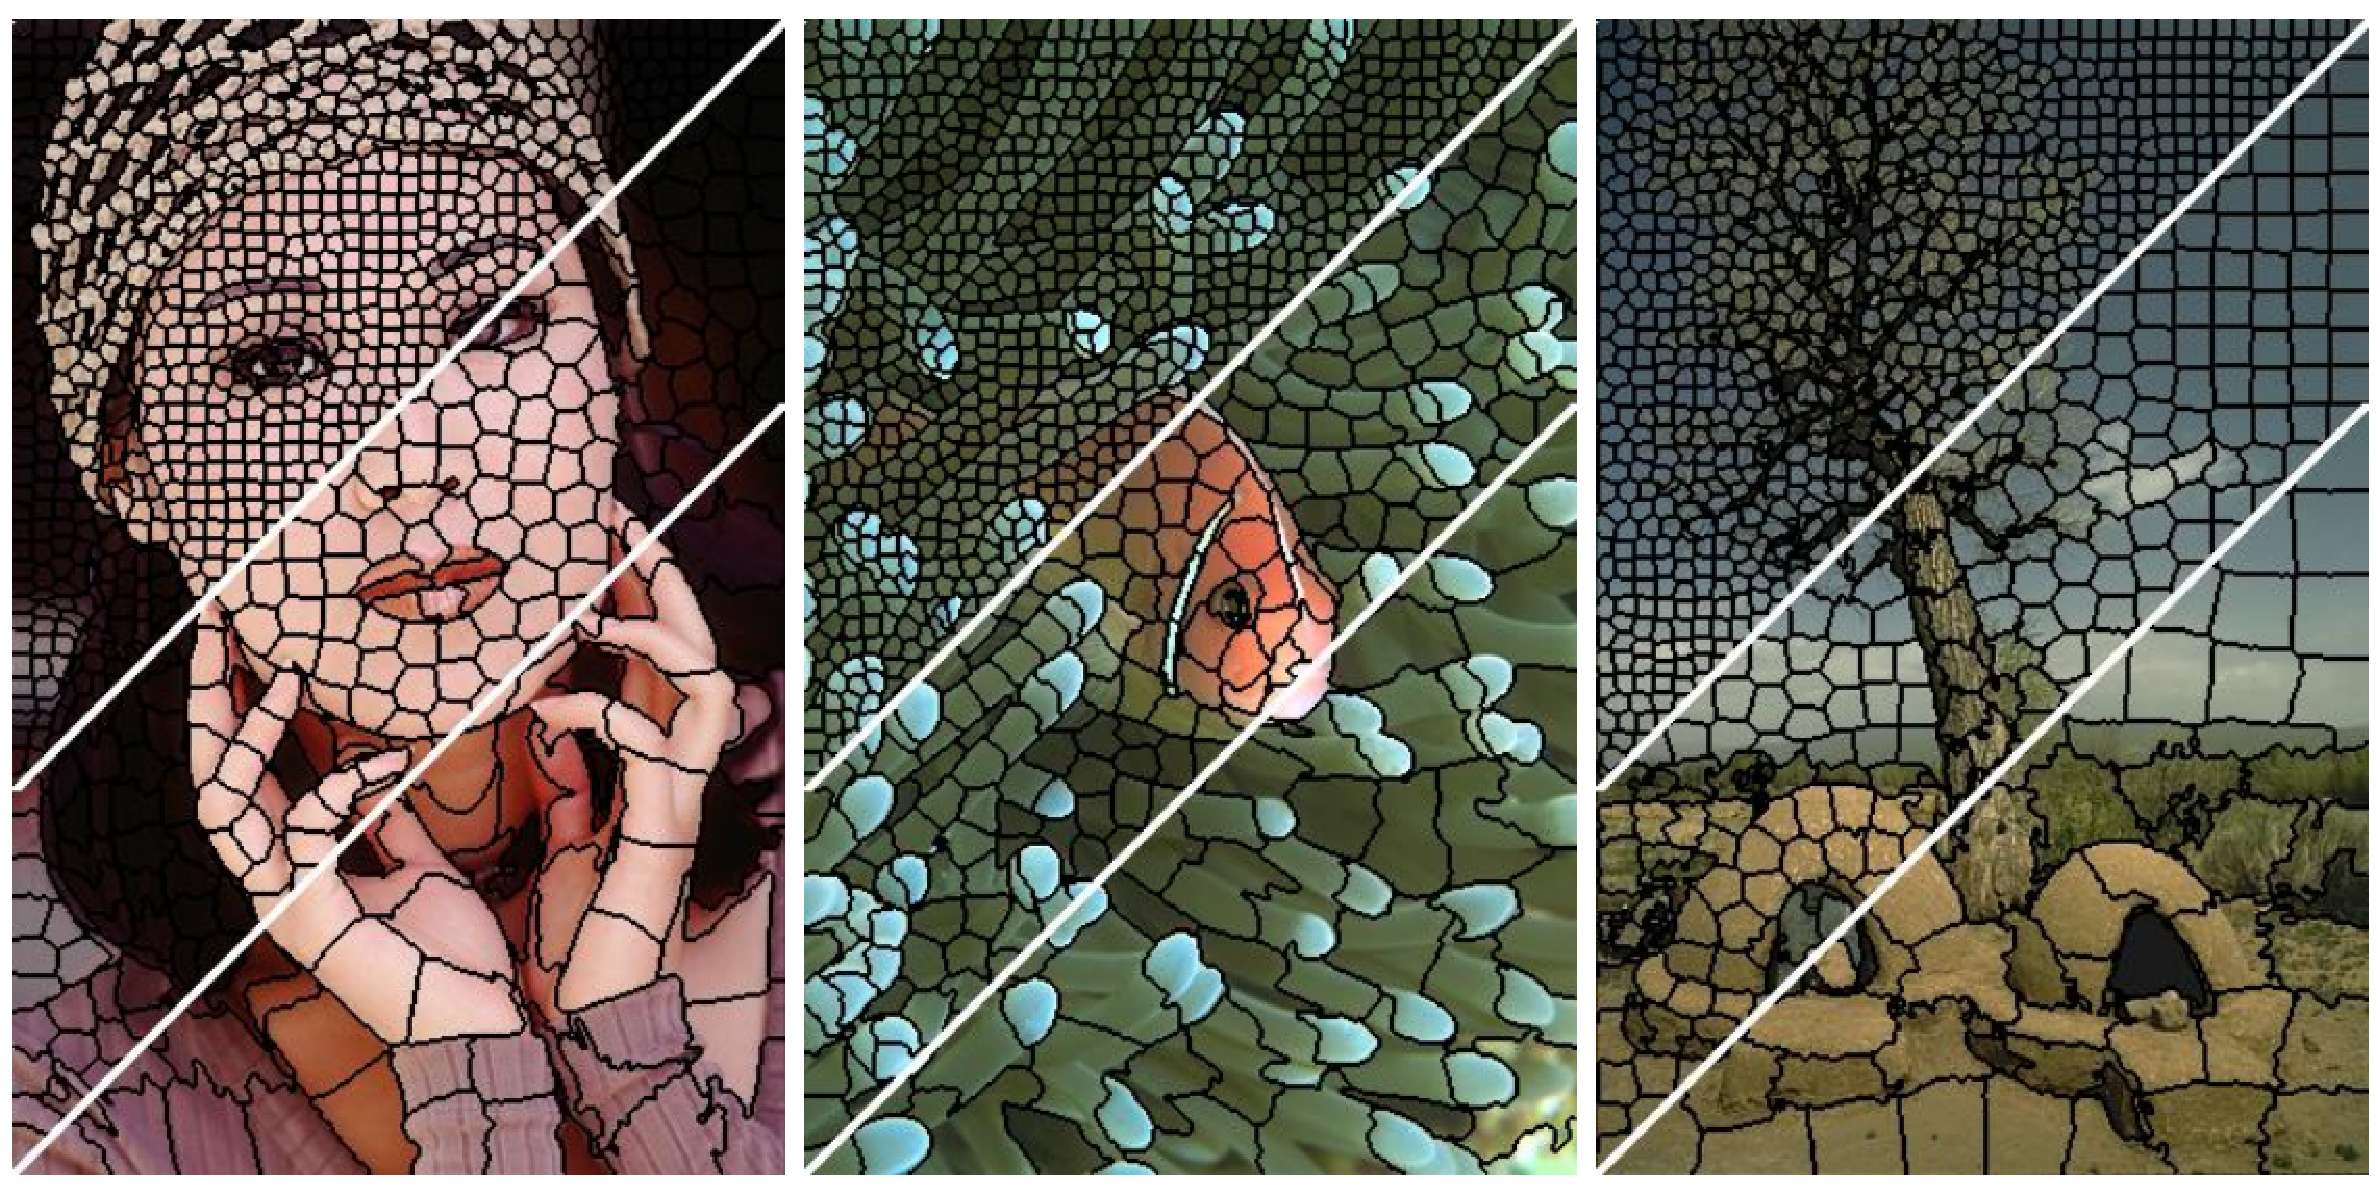
\includegraphics[width=0.8\textwidth]{figures/slic}
  \caption{SLIC 算法分割成尺寸为$64$,$256$ 和$1024$ 的超像素单元}\label{fig:slic}
\end{figure}

SLIC 算法将彩色图像转化为CIELAB颜色空间和XY坐标下的5维特征向量,即位于$(x,y)$ 处的像元在CIELAB颜色空间表示为$[l,a,b,x,y]$ ,CIELAB 空间由LAB 色彩模型表征,$l$ 为亮度,$a,b$ 为色彩值。对有$N$ 个像素点的图像,预分割为$K$ 个相同尺寸的超像素,则每个超像素单元的大小为$N/ K$, 则相邻种子间的步长为$S = \sqrt{N/K}$ 。SLIC 的搜索范围限制为$2S*2S$,对于每个搜索到的像素点,分别计算它和该种子点的距离,包括颜色距离和空间距离。距离计算方法如下
\begin{equation}
  \label{eq:2-5}
  \begin{split}
  d_c &= \sqrt{(l_j-l_i)^2 + (a_j-a_i)^2 + (b_j - b_i)^2} \\
  d_s &= \sqrt{(x_j-x_i)^2 + (y_j-y_i)^2} \\
  D &= \sqrt{(\frac{d_c}{N_c})^2 + (\frac{d_s}{N_s})^2} 
  \end{split}
\end{equation}
式中,$d_c$ 表示颜色距离,$d_s$ 表示空间距离, $N_s$ 表示类内最大空间距离,定义为
\begin{equation}
  \label{eq:2-6}
  N_s = S = \sqrt{N/K}
\end{equation}
$N_c$ 为最大的颜色距离,取值随具体的图片而定,实验中一般取一个固定常数$m$ (取值范围为$(1\leq m \leq 40)$,一般取$10$。$D$ 表示总距离,即最终的距离度量为:
\begin{equation}
  \label{eq:2-7}
  D = \sqrt{(\frac{d_c}{m})^2 + (\frac{d_s}{S})^2} 
\end{equation}
通过迭代优化直至误差收敛即可完成图像的超像素分割。图~\ref{fig:slic} 所示为基于SLIC 算法分别将图像大约分成$64$,$256$ 和$1024$ 三个尺寸的结果。



\subsection{模糊聚类方法概述}
\label{subsec:chap02-1-2}
向对象的模


本模板不再预先装载任何绘图包(如 \textsf{pstricks,pgf} 等),完全由你自己来决定。
个人觉得 \textsf{pgf} 不错,不依赖于 Postscript。 此外还有很多针对 \LaTeX{} 的
GUI 作图工具,如 XFig(jFig), WinFig, Tpx, Ipe, Dia, Inkscape, LaTeXPiX,
jPicEdt, jaxdraw 等等。

强烈推荐《\LaTeXe 插图指南》!关于子图形的使用细节请参看 \textsf{subfig} 的说明文档。

一般图形都是处在浮动环境中。之所以称为浮动是指最终排版效果图形的位置不一定与源文
件中的位置对应\footnote{This is not a bug, but a feature of \LaTeX!},这也是刚使
用 \LaTeX{} 同学可能遇宏包,
%它提供了 \texttt{[H]} 参数。比如图~\ref{fig:xfig1}。
%\begin{figure}[H] % use float package if you want it here
%  \centering
%  
\includegraphics{hello}
%  \caption{利用 Xfig 制图}
%  \label{fig:xfig1}
%\end{figure}

\section{基于神经网络的遥感影像分割方法}
\label{sec:chap02-2}

一般图形都是处在浮动环境中。之所以称为浮动是指最终


